%//------ Section 04 -------------------------------------------------------------------------------------------------
\chapter{Analysis of the correlated production of strange hadrons}
\label{chap:CorrelatedAnalysis}
%//-----------------------------------------------------------------------//

Following the mass measurement of multi-strange baryons in  \chap\ref{chap:CPTAnalysis}, the present work is complemented by a second analysis. Similarly to the first one, the latter pushes the limits of the LHC Run-2. It proposes to correlate the production of hyperons -- and most particularly, \rmOmega -- and other particles produced in the event. 

\section{Introduction}

The Quark Gluon Plasma (QGP) is studied experimentally for more than two decades now, from the first hints of its existence at the SPS in the years 2000's to its fine characterisation at LHC nowadays (\Sec\ref{sec:QGP}). It is explored through the study of its signatures and, for a long time, was considered as a well understood medium. Recently, it has been observed that small systems exhibit most of the signs usually attributed to the QGP: long range correlation in the lowest multiplicity pp collisions\cite{alicecollaborationALICESeesRidge}, collective flow \cite{cmscollaborationEvidenceCollectiveMultiparticle2015}\cite{alicecollaborationAnisotropicFlowFlow2022}, heavy quarkonia suppression \cite{singhCharmoniumSuppressionUltrarelativistic2022}\footnote{Only the thermal photons and jet quenching signatures have not been observed in small systems (yet), whereas they are present in heavy-ion collisions. The investigation of these two signatures in small systems will be further examined in the LHC Run-3 and Run-4 \cite{vanleeuwenHighlightsALICE59th}.}. This observation questions the very foundations of the QGP concept: either the QGP physics picture in heavy ion collisions must be re-designed and further rooted on pp collisions, or conversely, the QCD physics in small systems should be extended with new features to introduce collectivity. One way or the other, a better description of the pp and heavy-ion collision dynamics appears as an absolute must, in order to a continuum of physics.

\begin{figure}[t]
%\centering
\hspace*{-1.25cm}
\subfigure[]{
	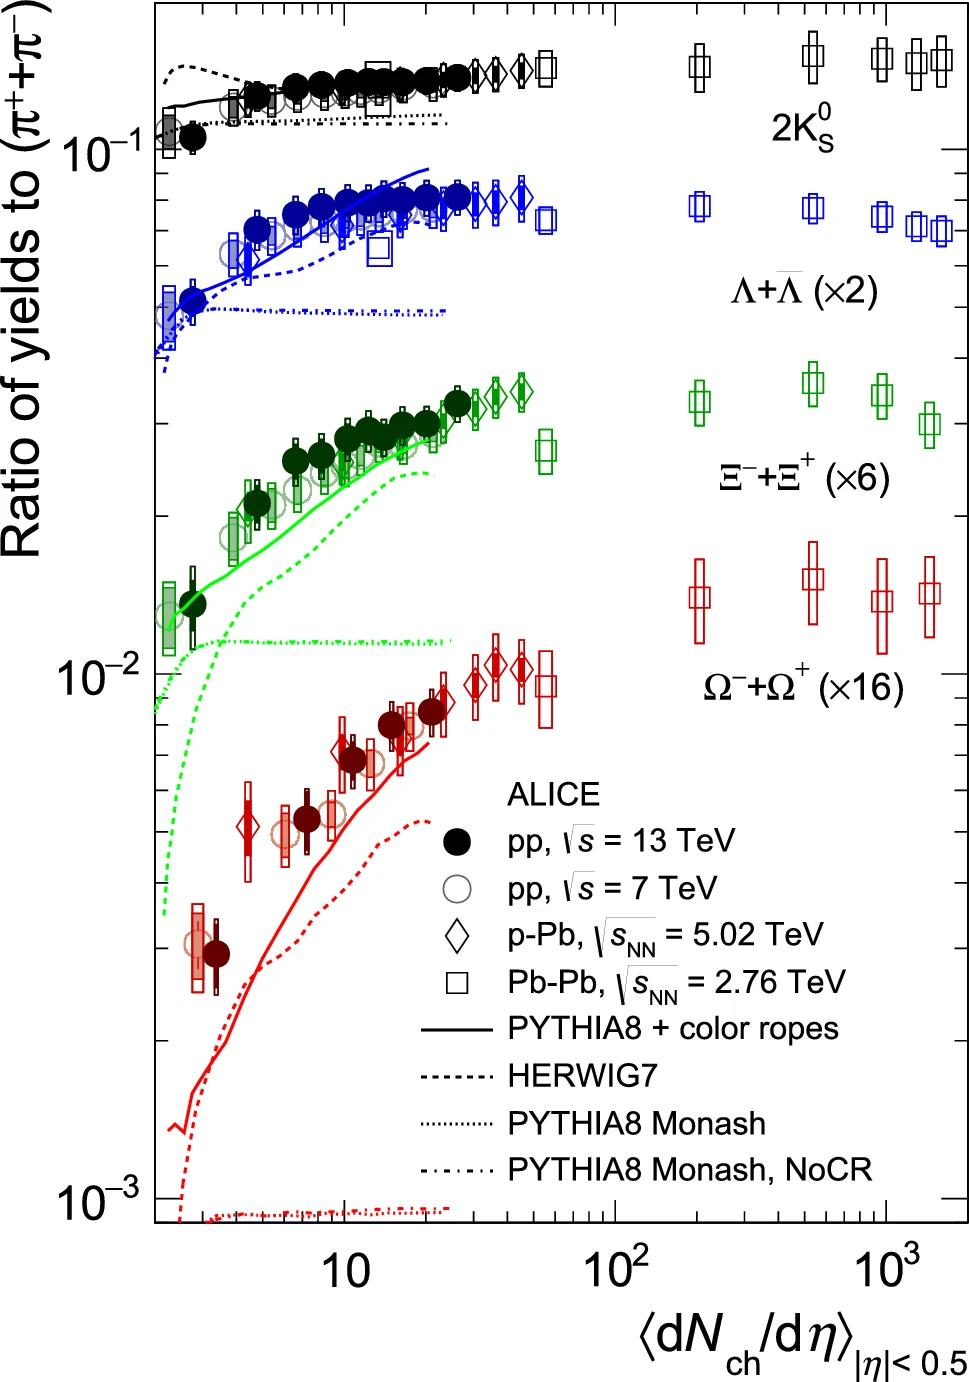
\includegraphics[width=0.55\textwidth, valign=t]{Figs/Chapter6/img.jpg}
	\label{fig:PythiaVsStrangenessEnhancement}
} 
\subfigure[]{
	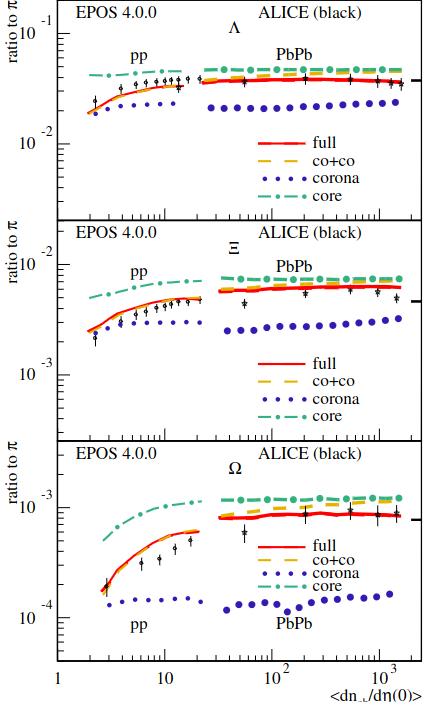
\includegraphics[width=0.6\textwidth, valign=t]{Figs/Chapter6/StrangenessEnhancement_CoreCorona.png}
	\label{fig:EposVsStrangenessEnhancement}
} 
\caption{Integrated strange hadrons-to-pions yield ratio as a function of the average charged particle multiplicity at mid-rapidity in ALICE, compared to different MC predictions. On the left, it is measured in pp at \sqrtS = 7 and 13 \tev, p-Pb at \sqrtSnn = 5.02 \tev, Pb-Pb collisions at \sqrtSnn = 2.76 \tev , and compared to \Pythiaeight and \Herwig\cite{acharyaMultiplicityDependencePi2020}; on the right, these are measurements in pp at \sqrtS = 7 \tev and Pb-Pb collisions at \sqrtSnn = 2.76 \tev, with different predictions from \Epos \cite{wernerCorecoronaProcedureMicrocanonical2023}.}
	\label{fig:MCModelStrangenessEnhancement}
\end{figure}

One of the key historical signatures of QGP is the strangeness enhancement which consists in the enhanced yield of multi-strange hadrons in heavy ion collisions with respect to small systems (\Sec\ref{subsec:StrangenessEnhanement}). Such yields also scale smoothly with the charged particle multiplicity in pp collisions (\Sec\ref{subsec:ComparisonPP}, \fig\ref{fig:StrangenessEnhancement}). Different models using fundamentally different mechanisms manage to reproduce qualitatively this trend (\fig\ref{fig:MCModelStrangenessEnhancement}). On one hand, \Pythia models the quark hadronisation using the Lund Strings; these correspond to gluon fields, that break whenever the string tension energy is high enough and thus leading to the formation of hadrons, similarly as in \fig\ref{fig:QuarkFragmentation}. Both pp and heavy-ion collision physics originate from the interaction of these strings, \ie this approach assumes the absence of a QGP. On the other hand, \Epos relies on a core-corona model: a dense core hosting a QGP-like collective medium, surrounded by a hadron gas corona \cite{wernerAnalysingRadialFlow2014}. So far, neither of these approaches has been able to provide an unambiguous explanation on the emergence of collective phenomena in small systems. Further experimental inputs are required in order to distinguish them, and finally identify the hadron production mechanisms. 

A way to shed more light on the situation is to perform more multi-differential study, typically of the angular and rapidity correlations between different hadron species. These bring informations on the quark production, and consequently on the hadronisation. Two hadrons produced out of the breaking of a colour string into a quark-antiquark pair, as modeled by \Pythia, should exhibit a strong local correlations. On the other hand, if the quarks are produced in the early stage of the collision -- the so-called \say{prehadrons} in \Epos framework \cite{wernerCorecoronaProcedureMicrocanonical2023} -- and hadronise later, that correlation should vanish.

\begin{figure}[t]
\centering
%\hspace*{-1.25cm}
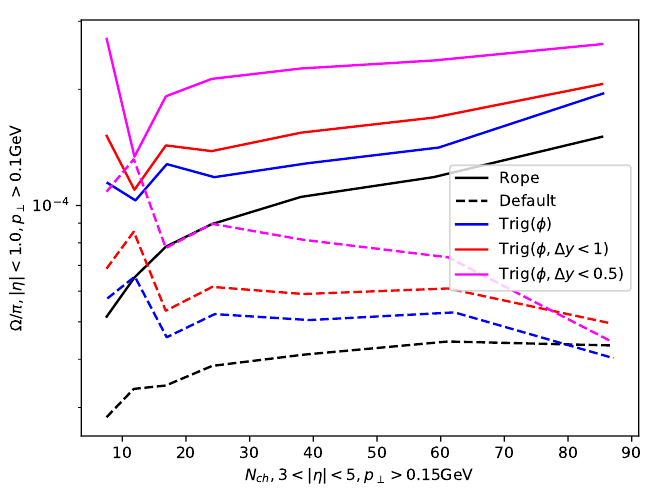
\includegraphics[width=0.8\textwidth]{Figs/Chapter6/PredictionPythia_Bierlich.png}
\caption{\Pythiaeight predictions for the \rmOmega-to-\rmPiPM yield ratio as a function of the charged particle multiplicity in pp collisions at \sqrtS =  13 \tev, in presence of a \rmPhiMes resonance (colour lines) or not (black line). The default \Pythia configuration (\Pythiaeight, tune: Monash 2013) is indicated in dashed line, whereas the full curves represent the case with the colour ropes enabled.}
	\label{fig:PredictionPythia_Bierlich}
\end{figure}

One example of such measurement comes from the \Pythia experts; since strangeness is conserved by the strong interaction, the number of strange hadrons is expected to be exactly compensated by the number of anti-strange hadrons, leading to a correlation between these hadrons\footnote{As a side note, since all the strange hadrons are correlated, one can control to some extent the strangeness content within an event using a trigger on strange particle, \rmXi or \rmOmega for example.}. In particular, within the standard Lund string framework, multi-strange baryons can be produced through a diquark-antidiaquark string breaking. However, the \say{recent} developments towards heavy-ion collisions -- namely the colour reconnection and colour rope \cite{christiansenStringFormationLeading2015}\cite{bierlichEffectsOverlappingStrings2015a}\cite{adolfssonQCDChallengesPp2020} -- offer new production mechanisms. As a consequence, it is predicted that i) the \rmOmega abundancy increases in presence of a \rmPhiMes in the event, and ii) this enhancement gets more prominent as the gap in rapidity between these two particles decreases.

So far, no such correlation has ever been measured. A similar observable has been studied recently \cite{adolfssonStudyXiHadron2020}, that analyses the angular correlations between the multi-strange baryon \rmXiPM and \pOrPbar, \rmPiPM, \rmKPM, \rmLambdaPM, \rmXiPM itself. It was not extended to \rmPhiMes resonance nor repeated with \rmOmega baryons, though. Therefore, this analysis aims to check this prediction via the measurement of correlated production of \rmOmega and \rmPhiMes over all the pp collisions at a centre-of-mass energy of 13 \tev collected throughout the LHC Run-2 by ALICE. In order to reduce as much as possible the background contamination, such measurement requires a trigger with a high purity, and thus good control capabilities over the amount of signal and the background for the trigger. For that reason and contrarily to the \Pythia's prediction, the trigger is on the \rmOmega particles and not the \rmPhiMes, the former offering a more governable purity.

Since the \rmXi baryon is much more produced than the \rmOmega, two measurements are performed : first, the correlated production of \rmXi and \rmPhiMes, and then the one of \rmOmega and \rmPhiMes. In this way, the feasibility of such measurement can be checked on the \rmXi, and if so, it will be repeated with the \rmOmega.\\

By design, this kind of analysis relies on two categories of particles: the \textit{trigger particles}, which is then correlated to the particles of interest in the event, the \textit{associated particles}. In the present chapter, the term \textit{trigger particle} designates either a \rmXi or a \rmOmega baryon, and the \textit{associated particle} corresponds to the \rmPhiMes resonance.


\section{Data samples and event selection}

\subsection{The data samples}

Considering their relatively low yield -- about $ 2 \times 10^{-2}$ \rmXi and $\sim 1.85 \times 10^{-3}$ \rmOmega, and $\sim 3.8 \times 10^{-2}$ \rmPhiMes at mid-rapidity \cite{alicecollaborationProductionLightflavorHadrons2020} -- the correlation between these particles requires all the data available. Therefore, this second analysis employs the same real and simulated data samples as in the first one, in \chap\ref{chap:CPTAnalysis}. It means that all pp collisions at centre-of-mass energy of 13 \tev collected in 2016, 2017 and 2018 are put to use (\Sec\ref{subsec:DataSamples}). 

Contrarily to the first analysis, this one exploits data in AOD format, as it does not necessitate such a fine control over the data reconstruction. The analysed events also come from the second reconstruction cycle, the pass-2.

\subsection{The event selection}

All the event selections employed in the first analysis (\Sec\ref{subsec:EventSelection}) are also applied here. These are complemented by an additional requirement on the type of event.

The behaviour of the hadronic interactions at high energies is typically described by the Regge theory\cite{collinsIntroductionReggeTheory1977}. There exists two classes of interaction: the elastic collisions -- when the initial and final states of the interaction are the same -- and inelastic (\INEL) collisions, that involve the production of new particles. The latter subdivides into two categories: the diffractive and non-diffractive processes. The former combines single and double diffractive processes. Within the framework of the Regge theory, the diffractive processes occur respectively when either or both incoming protons become an excited system -- due to the exchange of Pomerons --, that later decay into stable final-state particles emitted close to the mother direction, \ie close to beam, at very forward rapidity \cite{alicecollaborationMeasurementInelasticSingle2013}.

This analysis focuses on hadrons produced in inelastic collisions at mid-rapidity, hence originating \textit{a priori} from non-diffractive processes. Experimentally, this kind of inelastic collisions are selected by requiring, at least, one reconstructed SPD tracklet in $\abspseudorap < 1 $. This condition is commonly refered as \INELZero\footnote{Note that \INELZero events do not correspond to the total number of inelastic collisions \INEL, due to the acceptance and efficiency of the \INELZero condition, the beam-induced background selections, the number of un-reconstructed events (because no preliminary primary vertex could be formed for example, \Sec\ref{subsubsec:PreliminaryVertex}). In fact, for MB$_{\rm AND}$, the \INELZero encompasses about 76.3$_{-0.8}^{+2.2}$\% of the total number of inelastic collisions \cite{alicecollaborationALICEDataPreparation2023}.}.\\

\begin{table}[t]
    \centering
    \begin{tabular}{c|ccccc}
    \noalign{\smallskip}\hline \noalign{\smallskip}
    Multiplicity Class & \upperRomannumeral{1} & \upperRomannumeral{2} & \upperRomannumeral{3} & \upperRomannumeral{4} & \upperRomannumeral{5} \\
	\sigmaIdx[]/\sigmaIdx[\INELZero] & 0-0.01\% & 0.01-0.1\% & 0.1-0.5\% & 0.5-1\% & 1-5\% \\	        
	$\langle \dNchdeta \rangle$ & $35.37_{-0.86}^{+0.92}$ & $30.89_{-0.51}^{+0.57}$ & $26.96_{-0.30}^{+0.37}$ & $24.23_{-0.30}^{+0.36}$ & $20.02_{-0.22}^{+0.27}$ \\
	\noalign{\smallskip}\hline \noalign{\smallskip}
	Multiplicity Class & \upperRomannumeral{6} & \upperRomannumeral{7} & \upperRomannumeral{8} & \upperRomannumeral{9} & \upperRomannumeral{10} \\
	\sigmaIdx[]/\sigmaIdx[\INELZero] & 5-10\% & 10-15\% & 15-20\% & 20-30\% & 30-40\% \\
	$\langle \dNchdeta \rangle$ & $16.17_{-0.18}^{+0.22}$ & $13.77_{-0.16}^{+0.19}$ & $12.04_{-0.14}^{+0.17}$ & $10.02_{-0.11}^{+0.14}$ & $7.95_{-0.09}^{+0.11}$ \\
	\noalign{\smallskip}\hline \noalign{\smallskip}
	Multiplicity Class & \upperRomannumeral{11} & \upperRomannumeral{12} & \upperRomannumeral{13} & & \\
	\sigmaIdx[]/\sigmaIdx[\INELZero] & 40-50\% & 50-70\% & 70-100\% & & \\
	$\langle \dNchdeta \rangle$ & $6.32_{-0.07}^{+0.09}$ & $4.50_{-0.05}^{+0.07}$ & $2.55_{-0.03}^{+0.04}$ &  &  \\
    \noalign{\smallskip}\hline \noalign{\smallskip}
    \end{tabular}
    \caption{Event multiplicity classes, with the corresponding fraction of the total inelastic cross section \INELZero (\sigmaIdx[]/\sigmaIdx[\INELZero]) and average charged particle multiplicity at mid-rapidity, $\langle \dNchdeta \rangle$. Table taken from \cite{alicecollaborationEnhancedProductionMultistrange2017}\cite{alicecollaborationPseudorapidityTransversemomentumDistributions2016}.}
    \label{tab:MultiplicityClasses}
\end{table}

Moreover, two estimators can be considered for the multiplicity determination: the total charge deposited in the VZERO scintillator arrays in $-3.7 < \eta < -1.7$ and $2.8 < \eta < 5.1$ (VZERO-M amplitude, \Sec\ref{subsubsec:EventMultDependence}); the number of reconstructed SPD tracklets in $\abspseudorap < 1$ ($\rmNTracklet^{\abspseudorap < 1}$). Although the choice between these two estimators seems innocent/arbitrary, notice that they cover different pseudo-rapidity regions: the former estimates the multiplicity (at mid-rapidity) based on the energy deposited at forward rapidity, while the latter counts the number of tracklets at mid-rapidity. This difference may have some implications. Since the observable is a yield ratio at mid-rapidity, the considered particle and/or its decay products may contribute to the number of reconstructed SPD tracklets, thus self-biasing the multiplicity event. In general, the separation between the region of interest and the volume covered by the multiplicity estimator should be as large as possible, in order to avoid or limit this auto-correlation. For that reason, the VZERO-M is taken as default multiplicity estimator. 

It follows that the events are divided into ten multiplicity classes, presented in \tab\ref{tab:MultiplicityClasses}. The \Sec\ref{sec:CascadeResonanceCorrelationAnalysis} will show that the reconstruction of cascade and a \rmPhiMes resonance in the same event requires at least five tracks. Therefore, the correlations between these two hadrons are measured for events comprised between the 50\% with the lowest multiplicity to the 1\% with the highest multiplicity, 


\section{Analysis of the multi-strange baryon-\rmPhiMes correlation}
\label{sec:CascadeResonanceCorrelationAnalysis}

\subsection{The correlation function}

The objective is to measure the correlation between a multi-strange baryon, either \rmXiPM or \rmOmegaPM, and a \rmPhiMes meson. Their correlation is evaluated by associating them in pairs, and observing how the pair population is distributed according to a given variable. More precisely, the focus here is on the correlated yield of \rmPhiMes meson in events containing, at least, one multi-strange baryon. Therefore, the observable should be the per-trigger yield of the \rmPhiMes meson as a function of the difference in \pT, rapidity, azimuthal angle between the trigger particle and the associated particles, and the multiplicity of the event, 

\begin{equation}
\frac{1}{N_{\text{trigger}}} \cdot \dNXdX{pairs}{$y$} = \frac{1}{\dNXdy{cascade}} \cdot \dNXdX{pairs}{$y$} \left(\Delta \pT, \Delta \varphi, \Delta y, \text{multiplicity} \right),
\label{eq:IdealCorrelationFunction}
\end{equation}
where the $N_{\text{pairs}}$ corresponds to the number of cascade-\rmPhiMes pairs.\\

It will become clear in the next sections that a multi-differential observable such as in \eq\ref{eq:IdealCorrelationFunction} cannot be measured currently with the LHC Run-2 data, due to the lack of statistics. Nonetheless, this correlation may still be investigated, although less differentially. Along this line, this analysis proposes to measure the per-trigger yield as a function of one variable at a time, \ie
\begin{align}
&\frac{1}{\dNXdy{cascade}} \cdot \dNXdXdy{pairs}{$\Delta y$},\\
&\frac{1}{\dNXdy{cascade}} \cdot \dNXdXdy{pairs}{$\Delta \varphi$},\\
&\frac{1}{\dNXdy{cascade}} \cdot \dNXdXdy{pairs}{$\Delta \pT$}.
\end{align}\\

A few words on the analysis strategy before proceeding. Therefore, only events containing a \rmXi or \rmOmega candidate are selected; from these, the particles of interest are reconstructed using the selections in \Sec\ref{subsec:ResonanceSelections}. After calculating the invariant mass of each candidate, they are sorted as a function of their \pT\footnote{This is necessary in order to correct for the detector acceptance and the reconstruction efficiency (\Sec\ref{subsec:AccEff}).} and -- only for the particles of interest -- the difference of rapidity $\Delta y$, azimuthal angle $\Delta \varphi$ and transverse momentum $\Delta \pT$ with respect to the trigger particle. The yields of both species are extracted from their respective invariant mass distributions, for each \pT, $\Delta \pT$, $\Delta y $ and $\Delta \pT$ bins, as presented in \Sec\ref{subsec:CascadeResonanceSignalExtraction}. 

In the present measurement, the associated particles comprise solely the \rmPhiMes. However, the analysis has been designed in view of extending the correlations to other kind of hadrons, namely \pOrPbar, \rmPiPM, \rmKPM, \rmKstarZero, \rmKzeroS, \rmLambdaPM, \rmXiPM and \rmOmegaPM.

\begin{table}[h]
    \centering
    \begin{tabular}{>{\centering\arraybackslash}b{1.5cm}@{\hspace{0.3cm}} >{\centering\arraybackslash}b{1.75cm}@{\hspace{0.3cm}} >{\centering\arraybackslash}b{2.85cm}@{\hspace{0.3cm}} >{\centering\arraybackslash}b{3.6cm}@{\hspace{0.3cm}} >{\centering\arraybackslash}b{2.5cm}@{\hspace{0.3cm}} >{\centering\arraybackslash}b{1cm}@{\hspace{0.3cm}}}
    \noalign{\smallskip}\hline\noalign{\smallskip}
	Particle & Quark content & Mass (\mmass) & Lifetime \cTau (cm) or Width $\Gamma$ (\mmass) & Dominant decay channel & B.R.\\	
    \noalign{\smallskip}\hline \noalign{\smallskip}
    	
	\rmPhiMes & $s \bar{s}$ & $1019.461 \pm 0.020$ & $\Gamma = 4.249$ & \rmKplus \rmKminus & 49.1\%\\
	
    \noalign{\smallskip}\hline \noalign{\smallskip}
    
    \rmLambda (\rmAlambda) & $u d s$ ($\bar{u}\bar{d}\bar{s}$) & $1115.683 \pm 0.006$ &  $\cTau = 7.89$ & \proton \piMinus (\pbar \piPlus) & 63.9\% \\
    
    \noalign{\smallskip}\hline \noalign{\smallskip}    
    
    \rmXiM (\rmAxiP) & $dss$ ($\bar{d}\bar{s}\bar{s}$) & $1321.71 \pm 0.07$ & $\cTau = 4.91$ & \rmLambda \piMinus (\rmAlambda \piPlus) & 99.9\% \\	
    \noalign{\smallskip}\hline \noalign{\smallskip}
    
	\rmOmegaM (\rmAomegaP) & $sss$ ($\bar{s}\bar{s}\bar{s}$) & $1672.45 \pm 0.23$ & $\cTau = 2.461$ & \rmLambda \rmKminus (\rmAlambda \rmKplus) & 67.8\%\\    
    \noalign{\smallskip}\hline\noalign{\smallskip}
    \end{tabular}
    \caption{A few characteristics, as of 2023, of the \rmLambda, \rmXi, \rmOmega hyperons and the \rmPhiMes meson resonance: quark content, mass, relative mass difference values with their associated uncertainties and their dominant decay channel as well as the corresponding branching ratio \cite{particledatagroupReviewParticlePhysics2022}.}\label{tab:ResonanceV0CascPDGMass}
\end{table}

The multi-strange baryons being already introduced in details in \chap\ref{chap:V0CascReconstruction} and \chap\ref{chap:CPTAnalysis}, we will be concentrating on the \rmPhiMes resonance. As presented in \tab\ref{tab:ResonanceV0CascPDGMass}, it has a mass of 1019.461 \mev and a width of 4.249 \mev, equivalent to a lifetime of approximately 46 \fm. It mainly decays via strong interaction into a pair of oppositely charged kaons with a branching ratio of 49.1\%, $\rmPhiMes \rightarrow \rmKplus \rmKminus$, as depicted in \fig\ref{fig:ResonanceDecay}. In the following, the \rmPhiMes will be studied in this decay channel.

The \rmPhiMes resonance is reconstructed by forming pairs of oppositely charged tracks;  similarly to the V0s, the positively charged daughter is called the \textit{positive} particle, the other the \textit{negative} particle. As a consequence of the strong nature of the decay, its short flight distance makes the decay vertex undistinguable from the primary interaction point. Thereby, the misassociated pairs cannot be discarded using geometrical selections -- as opposed to the topological reconstruction of V0s and cascades --, leading to a substantial combinatorial background. This is the reason why it was decided to consider the multi-strange baryons as trigger particles, instead of the \rmPhiMes resonance meson. This background can be evaluated and subtracted by making use of two techniques here, presented later in \Sec\ref{subsec:ResonanceSelections}. \\

\begin{SCfigure}[][h]
\centering
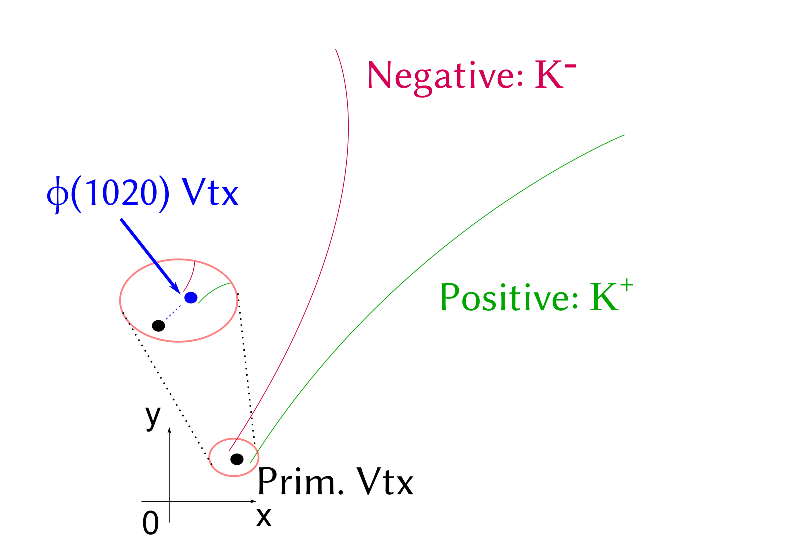
\includegraphics[width=0.65\textwidth]{Figs/Chapter6/Schema-PhiDecay.eps}
\caption{Scheme of the resonance decay of the \rmPhiMes meson. Modified version of the original figure \cite{maireFourTypesCascade2011}.}
	\label{fig:ResonanceDecay}
\end{SCfigure}


\subsection{Cascade candidate selections}

As in \chap\ref{chap:CPTAnalysis}, the identification of multi-strange baryons relies on their characteristic cascade decay channel. Their reconstruction therefore exploits the same topological and kinematic selection variables, \Sec\ref{subsec:TrackSelections} and \ref{subsec:V0CascSelections}. These are presented in \tab\ref{tab:TriggerParticleSelections}.

There is however one important difference with respect to the first analysis. While the latter measures the mass integrated over all the \pT bins\footnote{There is one exception in \Sec\ref{subsubsec:MassDependenceOnPt}, where the \pT-differential measurement of the mass is performed in order to check the stability of the results with the transverse momentum.}, the objective here is to extract the yield of both trigger and associated particles, these being obtained from their \pT-differential production rate. 

\begin{equation}
\dNdy = \int_{0}^{+\infty} \dNdptdy \text{d}\pT
\end{equation}

\begin{table}[t]
    \centering
    \begin{tabular}{c|c|c}
    \noalign{\smallskip}\hline \noalign{\smallskip}
    \bf Candidate variable & Selections \rmXiPM & Selections \rmOmegaPM \\
    \noalign{\smallskip}\hline \noalign{\smallskip}    
    Cascade \pT interval (\gmom) & \multicolumn{2}{c}{$0.6 < \pT < 6.5$} \\
    Cascade rapidity interval & \multicolumn{2}{c}{\absrap < 0.5} \\
    Competing mass rejection (\gmass) & \NoWay & > 0.008 \\
    MC association (MC only) & \multicolumn{2}{c}{Correct identity assumption} \\ 

    \noalign{\smallskip}\hline \noalign{\smallskip}
    \bf Track variable & Selections \rmXiPM & Selections \rmOmegaPM \\
    \noalign{\smallskip}\hline \noalign{\smallskip}
    Pseudo-rapidity interval & \multicolumn{2}{c}{\abspseudorap < 0.8} \\
    TPC refit & \multicolumn{2}{c}{\CheckGr} \\
    Nbr of crossed TPC readout rows & \multicolumn{2}{c}{ > 70} \\
    $\Nsigma^{\rm TPC}$ & \multicolumn{2}{c}{< 4} \\
    \multirow{ 2}{*}{Out-of-bunch pile-up rejection} & \multicolumn{2}{c}{at least one track with} \\
     & \multicolumn{2}{c}{ITS-TOF matching} \\
    
    \noalign{\smallskip}\hline \noalign{\smallskip}
    \bf Topological variable & Selections \rmXiPM & Selections \rmOmegaPM \\
    \noalign{\smallskip}\hline \noalign{\smallskip}
    
    \multicolumn{3}{l}{\textbf{V0}} \\
    V0 decay radius (\cm) & > 1.2 & > 1.1\\
    V0 cosine of pointing angle & \multicolumn{2}{c}{> 0.97}\\
    |$m$($V0$) - \mPDG\rmLambda| (\gmass) & \multicolumn{2}{c}{< 0.008} \\
    DCA proton to prim. vtx (\cm) & \multicolumn{2}{c}{> 0.03} \\
    DCA pion to prim. vtx (\cm) & \multicolumn{2}{c}{> 0.04} \\
    DCA V0 to prim. vtx (\cm) & \multicolumn{2}{c}{> 0.06} \\
    DCA between V0 daughters (std dev) & \multicolumn{2}{c}{< 1.5} \\
    \noalign{\smallskip}\hline \noalign{\smallskip}
    
    \multicolumn{3}{l}{\textbf{Cascade}} \\
    Cascade decay radius (\cm) & > 0.6 & > 0.5 \\
    Cascade Lifetime (\cm) & \multicolumn{2}{c}{< 3 $\times$ \cTau}\\
    DCA bachelor to prim. vtx (\cm) & \multicolumn{2}{c}{> 0.04} \\
    DCA between cascade daughters (std dev) & \multicolumn{2}{c}{< 1.3} \\
    Cascade cosine of pointing angle & \multicolumn{2}{c}{> 0.998} \\
    Bachelor-proton pointing angle (rad) & \multicolumn{2}{c}{> 0.04} \\
    
    \noalign{\smallskip}\hline \noalign{\smallskip}
    \end{tabular}
    \caption{Summary of the topological and track selections, as well as the associated cut values, used in the reconstruction of \rmXiPM and \rmOmegaPM in pp events at \sqrtS = 13 \tev. The \textit{competing mass rejection} refers to the removal of the background contamination from other mass hypotheses (\Sec\ref{subsubsec:InvariantMassSelection})}\label{tab:TriggerParticleSelections}
\end{table}

Thereby, the candidates are sorted as a function of their transverse momentum according to, for \rmXiPM baryons, thirteen \pT intervals: 
\begin{quote}
$\left[ 0.6 ; 1.0 \right) \gmom$,  $\left[ 1.0 ; 1.2 \right) \gmom$, $\left[ 1.2; 1.4 \right)\gmom$, $\left[1.4 ; 1.6 \right) \gmom$, $\left[ 1.6 ; 1.8 \right) \gmom$, 
$\left[ 1.8 ; 2.0 \right) \gmom$, $\left[ 2.0 ; 2.2 \right) \gmom$, $\left[ 2.2 ; 2.5 \right) \gmom$, $\left[ 2.5 ; 2.9 \right) \gmom$,  $\left[ 2.9 ;  3.4 \right) \gmom$,
$\left[ 3.4 ; 4.0 \right) \gmom$, $\left[ 4.0 ; 5.0 \right) \gmom$, $\left[ 5.0 ; 6.5 \right)\gmom$. 
\end{quote}

For what concerns the measurement of the \rmOmegaPM hyperons, due to their lower statistics, eight intervals are being used:
\begin{quote}
$\left[ 0.6 ; 1.0 \right) \gmom$,  $\left[ 1.0 ; 1.4 \right) \gmom$, $\left[ 1.4; 1.8 \right)\gmom$, $\left[1.8 ; 2.3 \right) \gmom$, $\left[ 2.3 ; 2.8 \right) \gmom$, $\left[ 2.8 ; 3.3 \right) \gmom$, $\left[ 3.8 ; 4.8 \right) \gmom$, $\left[ 4.8 ; 6.5 \right) \gmom$.
\end{quote}

\subsection{Resonance candidate selections}
\label{subsec:ResonanceSelections}

As explained in the header of this section, the \rmPhiMes meson candidates are reconstructed as a pair of \rmKplus and \rmKminus. Since the decay topology cannot be exploited to reduce the amount of combinatorial background, most of the selection criteria focus on the quality of daughter tracks\footnote{In this analysis, the focus is on the \rmPhiMes yield in presence of a multi-strange baryon. However, note that the same considerations would also apply in the case of the \rmKstarZero resonance, that decays strongly into a \rmKPM and a \rmPiPM at $\sim$100\%.}. These can be found in \tab\ref{tab:PhiSel}.

\begin{table}[h]
    \centering
    \begin{tabular}{c|c}
    \noalign{\smallskip} \hline \noalign{\smallskip}
    \bf Candidate variable & Selection criterion \\
    \noalign{\smallskip} \hline \noalign{\smallskip}    
    Resonance rapidity interval & \absrap < 0.5 \\
    MC association (MC only) & Correct identity assumption \\ 
    \noalign{\smallskip} \hline \noalign{\smallskip}
    \bf Track variable & Selection criterion \\
    \noalign{\smallskip} \hline \noalign{\smallskip}
    \pT interval (\gmom) & 0.15 < \pT < 20 \\
    Pseudo-rapidity interval & \abspseudorap < 0.8 \\
    ITS refit & \CheckGr \\
    TPC refit & \CheckGr \\
    Kink Topology & \NoWay \\
    $\Nsigma^{\rm TPC}$  & < 2 \\    
    $\Nsigma^{\rm TOF}$  (veto only) & < 3 \\    
    Nbr of crossed TPC readout rows & > 70 \\
	Fraction of crossed TPC readout & \multirow{2}*{$\geq$ 0.8} \\
	rows over findable clusters & \\
	Goodness of the TPC standalone track, $\chi_\textsc{TPC}^2 / N_{\rm cluster}$ & < 4 \\
	Global and TPC standalone track matching, $\chi_\textsc{TPC-CG}^2$ & < 36 \\
	Goodness of the ITS standalone track, $\chi_\textsc{ITS}^2 / N_{\rm cluster}$ & < 36 \\
	Nbr of associated SPD clusters & $\geq$ 1 \\
	DCA to prim. vtx (cm) & < 0.0105 + 0.035 \pT$^{-1.01}$ \\
	DCA to prim. vtx along z (cm) & < 2 \\
    \noalign{\smallskip} \hline \noalign{\smallskip}
    \end{tabular}
    \caption{Summary of the track and candidate selections used for the reconstruction of \rmPhiMes.}\label{tab:PhiSel}
\end{table}

Beyond the track selections in common with the hyperons (\Sec\ref{subsec:TrackSelections}), the track quality is improved by requiring a reduced $\chi^2$ up to 36 and 4, for the ITS and TPC standalone tracks respectively\footnote{The tighter selection on the goodness of the TPC standalone track is related to the fact that TPC is the main tracking device in ALICE and so, contributes the most to the track quality.}. The agreement between the TPC standalone track, constrained to the preliminary primary vertex (\Sec\ref{subsec:EventReco}), and global track is quantified by the so-called \textit{golden} $\chi^{2}$; its value should be smaller than 36. Along the same line, each track must have passed the final refit in the ITS, and be associated with at least one hit in the innermost ITS layers, the most granular detector in ALICE. To ensure a good momentum resolution, the fraction of found crossed TPC readout rows over the number of findable clusters must reach at least 80\%.  

Since the decay point cannot be resolved from the primary vertex, the formation of a resonance candidate uses primary tracks, contrarily to the V0 and cascade reconstruction. These are identified by imposing that their distance of closest approach to the primary vertex is smaller than a critical value. In particular, in the transverse plane, the latter is given by a \pT-dependent \textit{ad-hoc} formula in order to be even more selective.

Further combinatorial background is suppressed by applying PID criteria. It is required that each track agrees with a \rmKPM mass hypothesis within $n_{\sigma}^{\rm TPC} = \pm 3$. Whenever it matches a hit in the TOF detector\footnote{Since a substantial amount of particles do not reach the TOF detector or cannot be matched with a hit, the associated hadron identification capabilities can only be used as a veto, in complement to other PID informations; otherwise, this would drastically affect the track reconstruction efficiency.}, the time-of-flight informations supplement the selection on the nature of the decay daughter using the PID estimator in \eq\ref{eq:PIDestimatorTOF}, $n_{\sigma}^{\rm TOF}$.\\


Finally, any pair of tracks satisfying the above criteria and lying at mid-rapidity,  \absrap < 0.5, is considered as a \rmPhiMes meson candidate. Their measurement is performed in the following eight \pT intervals:
\begin{quote}
$\left[0.4; 0.8\right) \gmom$, $\left[0.8; 1.2\right) \gmom$, $\left[1.2; 1.8\right) \gmom$, $\left[1.8; 2.6\right) \gmom$, $\left[2.6; 3.4\right) \gmom$, $\left[3.4; 4.2\right)\gmom$, $\left[4.2; 5\right)\gmom$, $\left[5; 11\right) \gmom$.
\end{quote}


\subsection{The raw signal extraction}
\label{subsec:CascadeResonanceSignalExtraction}

\subsubsection{In the case of multi-strange baryons}

The raw signal extraction for the trigger particle follows the very same procedure as in the first analysis. Therefore, the invariant mass peak is modeled by a modified Gaussian (\eq\ref{eq:ModifiedGaus}), and the background by a linear function. The amount of raw signal and background are estimated by bin counting, over the same regions as in \Sec\ref{subsec:MassExtraction}. 

The \figs\ref{fig:InvMassXiMinusVPt}, \ref{fig:InvMassXiPlusVPt} show the invariant mass distribution in the different \pT intervals for \rmXiM, \rmAxiP, \rmOmegaM and \rmAomegaP respectively.

\begin{landscape}
\begin{figure}[h]
	\centering
	\includegraphics[width=1.45\textwidth]{Figs/Chapter6/InvMassFit\_VsPt\_XiMinus.eps}
\caption{Invariant mass spectra of the \rmXiM candidates in pp collisions at \sqrtS = 13 \tev, fitted by the combination of three Gaussian functions for the peak and a decreasing exponential function for the background. The amounts of signal and background have been obtained via bin counting in the peak (red area) and side-bands region (gray area).}
	\label{fig:InvMassXiMinusVPt}
\end{figure}

\begin{figure}[h]
	\centering
	\includegraphics[width=1.45\textwidth]{Figs/Chapter6/InvMassFit\_VsPt\_XiPlus.eps}
\caption{Invariant mass spectra of the \rmAxiP candidates in pp collisions at \sqrtS = 13 \tev, fitted by the combination of three Gaussian functions for the peak and a decreasing exponential function for the background. The amounts of signal and background have been obtained via bin counting in the peak (red area) and side-bands region (gray area).}
	\label{fig:InvMassXiPlusVPt}
\end{figure}

\end{landscape}

%\begin{table}[h]
%    \centering
%    \begin{tabular}{b{2cm}@{\hspace{1cm}} b{2.5cm}@{\hspace{0.5cm}} b{2cm}@{\hspace{0.5cm}} b{3cm}@{\hspace{0.5cm}} b{2cm}@{\hspace{0.1cm}}}
%    \noalign{\smallskip}\hline\noalign{\smallskip}
%	 & \multicolumn{4}{c}{\rmXiM (\rmAxiP)} \\	
%	\pT (\gmom) & Reduced $\chi^2$ & Raw signal & Background & Purity \\	
%    \noalign{\smallskip}\hline \noalign{\smallskip}
%    $\left[ 0.6 ; 1.0 \right)$ & 12.689 & 11.273 & 5.051 & 4.707\\
%    	$\left[ 1.0 ; 1.2 \right)$ &  1 237 666 & 1 168 882 & 65 232 & 63 842\\
%    	$\left[ 1.2; 1.4 \right)$ & 55 375 & 51 269 & 5758 & 5490 \\
%    	$\left[1.4 ; 1.6 \right)$ & 22.4 & 22.8 & 11.4 & 11.7 \\
%    	$\left[ 1.6 ; 1.8 \right)$ & 95.7\% & 95.8\% & 91.8\% & 92.1\% \\
%    $\left[ 1.8 ; 2.2 \right)$ & 1089 & 1059 & 245 & 243 \\
%    $\left[ 2.2 ; 2.5 \right)$ & 1089 & 1059 & 245 & 243 \\
%    $\left[ 2.5 ; 2.9 \right)$ & 1089 & 1059 & 245 & 243 \\
%    $\left[ 2.9 ; 3.4 \right)$ & 1089 & 1059 & 245 & 243 \\
%    $\left[ 3.4 ; 4.0 \right)$ & 1089 & 1059 & 245 & 243 \\
%    $\left[ 4.0 ; 5.0 \right)$ & 1089 & 1059 & 245 & 243 \\
%    $\left[ 5.0 ; 6.5 \right)$ & 1089 & 1059 & 245 & 243 \\
%    \noalign{\smallskip}\hline\noalign{\smallskip}
%    \end{tabular}
%    \caption{Results from the fit of the invariant mass distributions in \fig\ref{fig:InvMassCascades} concerning the samples of \rmXiM, \rmAxiP, \rmOmegaM and \rmAomegaP. Therefore, this table reports the reduced $\chi^{2}$, raw signal, background, ratio $S/B$, purity and signal significance.}\label{tab:FitQuantities}
%\end{table}

\subsubsection{In the case of \rmPhiMes meson}
\label{subsubsec:RawSignalExtractionPhiMes}

The invariant mass of each resonance candidate is calculated using the \eq\ref{eq:ResonanceInvMass} and making the assumption of a \rmKPM mass for both decay daughters. The top left \fig\ref{fig:InvMassPhiResVsPt} present the invariant mass spectra of the \rmPhiMes meson for every \pT intervals. 
\begin{align}
M_{\rm candidate}^2 \left[ \rmPhiMes \right] &= ( E_{\rm pos.} + E_{\rm neg.} )^2 - ( \vec{p}_{\rm pos.} + \vec{p}_{\rm neg.})^2 \\
&= \Big(\sqrt{ \vec{p}_{\rm pos.}^2 + m_{\rm pos.}^2} + \sqrt{ \vec{p}_{\rm neg.}^2 + m_{\rm neg.}^2}\Big)^2 - ( \vec{p}_{\rm pos.} + \vec{p}_{\rm neg.})^2\\
&= \Big(\sqrt{ \vec{p}_{\rm pos.}^2 + m_{\rm K^{+}}^2} + \sqrt{ \vec{p}_{\rm neg.}^2 + m_{\rm K^{-}}^2}\Big)^2 - ( \vec{p}_{\rm pos.} + \vec{p}_{\rm neg.})^2 \label{eq:ResonanceInvMass}
\end{align}
An excess of counts emerges around the tabulated mass of the \rmPhiMes, $\mPDG = 1019.461$ \mmass, on top of a smooth background. The latter dominates the invariant mass distribution, and derives \textit{a priori} mainly from combinatorics of the tracks. The origin of the background being known, it can thus be removed\footnote{Alternatively, one could try to find a functional form that describes correctly the shape of the background, as it was done in \chap\ref{chap:CPTAnalysis}. For instance, here, it could be modeled by a second order polynomial.}. The basic idea consists to reproduce the background shape by forming uncorrelated pairs of tracks. There exist two approaches\footnote{In fact, there also exist a third approach. These resonances are formed out of two oppositely charged, \ie unlike-charge, tracks. Particles of the same charge are uncorrelated with respect to the \rmPhiMes decay. Hence, by pairing like-charge tracks, \rmKplus\rmKplus and \rmKminus\rmKminus, the combinatorial background can be estimated. However, this procedure has been implemented in the analysis, and so will not be used.}:
\begin{itemize}
\item[$\bullet$] \textbf{Event mixing technique:} by definition, particles originating from different events could not have been produced together, and so are uncorrelated. Consequently, the association of tracks from different events should \textit{in principle} result in combinatorial background. This is core concept of event mixing.
Therefore, each positively charged track passing the above selections (\Sec\ref{subsec:ResonanceSelections}) gets paired to a negatively charged track from another event, under the exact same set of cuts, and vice versa. Each event is mixed with five other events at most.
In order to estimate correctly the combinatorial background, the mixing has to be performed between events with similar collision kinematics. To ensure that, it is required that i) the longitudinal position of their primary vertex agrees within a range of $\pm$ 1 \cm, and ii) their difference in terms of event multiplicity should be sufficiently low, such that they belongs to the same multiplicity class. Moreover, since the several events are involved in the mixing, the mixed-event invariant mass distribution needs to be normalised, such that it fits the same-event distribution in certain invariant mass region. This normalisation is usually performed far from the peak, in the side-bands regions purely populated by combinatorial background.
\item[$\bullet$] \textbf{Rotating procedure:} the excess of counts in the invariant mass distributions originates from correlated pairs of \rmKplus and \rmKminus due to the \rmPhiMes meson decay. If the correlation of the pair could somehow be broken, the invariant mass spectrum should be populated solely by combinatorial background. This can be achieved by considering the already formed pairs of kaons from the same event and rotating one of track by a significant amount, typically by an angle of 180\textdegree. 
\end{itemize}

\begin{figure}[t]
	\hspace{-2.cm}
%	\centering
	\includegraphics[width=1.35\textwidth, angle=0]{Figs/Chapter6/InvMassFit\_VsPt\_Resonance.eps}
\caption{Top left panel: Unlike-charge and mixed-event invariant mass distribution for \pT between 0.4 and 0.8 \gmom. The other panels: Invariant mass spectra of the \rmPhiMes meson candidates in pp collisions at \sqrtS = 13 \tev, fitted by the sum of a Voigt function for the peak and a linear function for the residual background. The amounts of signal have been obtained as explained in \Sec\ref{subsubsec:RawSignalExtractionPhiMes}, while the background has been obtained via bin counting in the region covered by the red area, that is 1.005 and 1.035 \gmass.}
	\label{fig:InvMassPhiResVsPt}
\end{figure}

The event mixing technique is taken as the default option, as it will later facilitate another part of the analysis \Sec\ref{subsec:EvtMixingCascPhi}. The rotating procedure is going to be used in the systematic study. 

Whatever the considered approach, the combinatorial background is subtracted from the invariant distribution, yielding to the \figs\ref{fig:InvMassPhiResVsPt}. The invariant mass now sits on top of a small residual background. The signal is separated from the background through a (log-)likelyhood method. 

The ideal signal for a resonance should exhibit a Breit-Wigner shape \cite{breitCaptureSlowNeutrons1936}. However, the invariant mass peak rather corresponds to the convolution of Breit-Wigner and Gaussian -- due to the smearing induced by the detectors response -- distributions, namely the Voigt profile in \eq\ref{eq:Voigt}. 

\begin{equation}
\dNdX{\mInv} = A \cdot \frac{\Gamma}{(2\pi)^{3/2} \sigma} \int\limits_{-\infty}^{\infty} \text{exp} \left[ -\frac{(\mInv - m')^2}{2\sigma^2} \right] \frac{1}{(m' - \mu)^2 + \Gamma^2/4} \text{d} m',
\end{equation}\label{eq:Voigt}
where:
\begin{itemize}
\item[$\bullet$] $A$ coincides with the integral of the function from $0$ to $+\infty$,
\item[$\bullet$] $\mu$ corresponds to the centre of the Voigt function,
\item[$\bullet$] $\Gamma$ is the resonance width,
\item[$\bullet$] and $\sigma$ describes the width of the Gaussian.
\end{itemize}

Only this function is considered for the peak description. Here, two types of Voigtian fits are considered: one with the resonance width fixed at the nominal value ($\Gamma = 4.249$ \mmass), the other where it is allowed to vary freely. Concerning the residual background, as in the first analysis, different shapes can be considered: constant, linear, exponential functions, second order polynomial. \\

If the fitting procedure converges, the signal and background are estimated. As the Voigt function (resonance case) does not decrease as fast as a Gaussian (multi-strange baryon case) with the distance to centre, the amount of raw signal and background have to be evaluated differently. In this context, the peak region is defined in $\left[1.005 ; 1.035\right] \gmass$, and contains most of the signal and some background. Therefore, the raw signal is obtained by counting the number of candidates in this region and subtracting the background population; the latter is given by the integral of the background function over the same region, hence $S_{\rm counting} = \left(S+B\right)_{\rm counting} - B_{\rm integral}$. The rest of the signal population sits outside the peak region, from 0.987354\footnote{It corresponds to $2 m_{\rm K^{\pm}} = 0.987354 \gmass$ with $m_{\rm K^{\pm}} = 0.493677 \gmass$ \cite{particledatagroupReviewParticlePhysics2022}. The population of \rmPhiMes cannot be found below this mass value because it is kinematically forbidden.} to $1.005$ \gmass and $1.035$ to $+\infty$ \gmass. Consequently, the integral of the Voigt function in these two regions provides an estimation of the missing signal population, which is then incorporated in the total raw signal $S = S_{\rm counting}\left( 1.005 ; 1.035 \right) + S_{\rm integral}\left( 0.987354 ; 1.005\right) + S_{\rm integral} \left( 1.035 ; +\infty\right)$\footnote{In the analysis, the peak function is not integrated to $+$ infinity, but rather up to a large mass value with respect to the \rmPhiMes mass -- that is 5 \gmass -- such that most of the missing raw signal has been taken into account.}.

\subsection{Fraction of background cascade}
\label{subsec:FractionOfBkgCascade}

As explained in the header of this section, the correlation between cascade and resonances goes through pairs of particle candidates. Thereby, as illustrated in \tab\ref{tab:CorrelationTab}, there exist four types of pairs depending on whether they are signal or background candidates.

\begin{table}[h]
\centering
\begin{tabular}{ | c | c | c | }
	\hline
	\backslashbox{\rmXiPM or \rmOmegaPM}{\rmPhiMes}
    & Signal candidate & Background candidate \\
	\hline
    Signal candidate & Signal-Signal & Signal-Background \\
    Background candidate & \cellcolor{red!50} Background-Signal & \cellcolor{red!50}Background-Background \\
	\hline
\end{tabular}
\caption{Four types of cascade-resonance correlation in the analysis, depending on the cascade and resonance candidates. The red cells represent the correlations with a background trigger candidate, that must be removed.}
\label{tab:CorrelationTab}
\end{table}


In the ideal case, only correlation between a true \rmXiPM or \rmOmegaPM and an actual \rmPhiMes should be observed. As explained in \Sec\ref{subsec:ResonanceSelections}, the contribution from the background resonances is already removed bin-by-bin first using an event mixing technique, and then the raw signal of \rmPhiMes is isolated from the residual background through a fit with a linear function. The only remaining source of correlation with background candidate comes from the multi-strange baryons. Considering the purity of the sample, the contribution of the cascade background candidates could be assumed as negligible. This means that
\begin{align}
\frac{1}{N_{\text{trigger}}} \cdot \dNXdXdy{pairs}{$X$} &= \left.\frac{1}{N_{\text{trigger}}(S)} \cdot \dNXdXdy{\rmPhiMes}{$X$}\right|_{(S)\ \textrm{trigger} -\  (S)\ \textrm{associated pairs}}\\
&\simeq \left.\frac{1}{N_{\text{trigger}}(S+B)} \cdot \dNXdXdy{pairs}{$X$}\right|_{(S+B)\ \textrm{trigger} -\  (S)\ \textrm{associated pairs}},
\end{align}
where $X$ corresponds to either $\Delta y$, $\Delta \varphi$ or $\Delta \pT$, $(S+B)$ signifies signal and background candidates, and $(S)$ is for pure signal candidates.\\

An attempt is made to get as precise as possible. To that end, two measurements are performed: one in which cascades in the peak region are correlated to resonance candidates, and another with cascades from the side-bands region instead. Each of them provides a set of invariant mass distributions for the associated particles as a function of their rapidity, azimuthal angle and/or transverse momentum gap with respect to the trigger particle. 

\begin{align}
\frac{1}{N_{\text{trigger}}} \cdot \dNXdXdy{\rmPhiMes}{$X$}&= \left.\frac{1}{N_{\text{trigger}}(S)} \cdot \dNXdXdy{\rmPhiMes}{$X$}\right|_{(S)\ \textrm{trigger} -\  (S)\ \textrm{associated pairs}}\\
&= \frac{1}{N_{\text{trigger}}(S+B) - N_{\text{trigger}}(B)} \cdot \left[ \left.\dNXdXdy{\rmPhiMes}{$y$}\right|_{(S+B)\ \textrm{trigger}} - \left.\dNXdX{\rmPhiMes}{$y$}\right|_{(B)\ \textrm{trigger}} \right].
\end{align}

\subsection{Acceptance and efficiency corrections}
\label{subsec:AccEff}

The raw signal quantifies the amount of multi-strange baryons or \rmPhiMes resonances reconstructed within the acceptance of the ALICE detector, and satisfying the selections in \tabs\ref{tab:CascadeSelections} and \ref{tab:PhiSel}. In fact, this quantity corresponds to a fraction of the total number of particles produced in the fiducial volume $\absrap < 0.5$ due to i) the limited acceptance of the detector that prevents the reconstruction of tracks within certain region of the ALICE apparatus (beyond $\abspseudorap < 0.8$, deadzones), and ii) the finite reconstruction and selection efficiencies of the cascade and resonance decays. This fraction can be estimated using MC simulations.

In principle, the correction on the raw signal breaks down into two terms, one for each of the aforementioned contributions: the \textit{acceptance}, that corresponds to the fraction of reconstructable particles in the fiducial volume among the total number of generated particles within the desired rapidity region ($\absrap < 0.5$), and the \textit{efficiency} given by the ratio of the number of reconstructed hadrons over the number of reconstructable ones in the same rapidity interval. The product of these two terms provides the acceptance and efficiency correction factors (\eq\ref{eq:AccEff}).

\begin{align}
\textrm{Acceptance} \times \textrm{Efficiency} &= \frac{N_{\rm generated\ in\ |y| < y_{\rm fid.}}^{\rm daughter\ in\ acc.}}{N_{\rm generated\ in\ |y| < 0.5}} \times \frac{N_{\rm reconstructed\ in\ |y| < y_{\rm fid.}}}{N_{\rm generated\ in\ |y| < y_{\rm fid.}}^{\rm daughter\ in\ acc.}}\label{eq:AccEff}\\
&= \frac{N_{\rm reconstructed\ in\ |y| < y_{\rm fid.}}}{N_{\rm generated\ in\ |y| < 0.5}}\label{eq:FinalAccEff}
\end{align}

For the sake of simplicity, instead of evaluating these correction factors individually, this analysis goes directly for the product of the two (\eq\ref{eq:FinalAccEff}). Since the above selections impact differently low-\pT and high-\pT candidates, these acceptance and efficiency correction factors do depend strongly on the transverse momentum. Therefore, they have to be determined for every \pT-bin. Moreover, note that the branching ratio of the considered particle stands as an upper bound for the reconstruction efficiency, and so for the acceptance $\times$ efficiency.\\

These corrections aim to compensate for the un-detected and/or un-reconstructed particles in the analysis. Hence, most of the measurements apply such corrections on both trigger and associated particles. While this makes sense in the latter case, it is more dubious for the former ones: by correcting the cascade raw signal, one increases basically the number of such hadrons in the analysis. Those being used as a trigger, it also amounts to increase the number of triggered events. Depending on whether those additional/corrected events contains a \rmPhiMes meson or not, whether they are reconstructed or not, whether they are correlated to the trigger particle or not, this will most certainly affect the estimation of the \rmXiPM-\rmPhiMes and \rmOmegaPM-\rmPhiMes correlations. If, as depicted in the left panel of \fig\ref{fig:TriggeredContribution}, such correlation in non-triggered event turns out to be small, the previous concerns may reasonably be neglected in first approximation. Conversely, in the configuration shown in the right panel of \fig\ref{fig:TriggeredContribution}, one should be extremely cautious on how to correct the trigger particle yield.

\begin{figure}[t]
\begin{minipage}[c]{0.4\linewidth}
\begin{align*}
\left[\begin{array}{>{\centering\arraybackslash}b{4.5cm}@{\hspace{0.2cm}}|>{\centering\arraybackslash}b{1.1cm}@{}}
      \cellcolor{green!50} & \cellcolor{red!50}\\
      \cellcolor{green!50} & \cellcolor{red!50}\textsc{\footnotesize T}\\
      \cellcolor{green!50} \textsc{\footnotesize T \& C} & \cellcolor{red!50}\textsc{\footnotesize \&}  \\  
      \cellcolor{green!50} & \cellcolor{red!50}\textsc{\footnotesize \cancel{C}} \\
      \cellcolor{green!50} & \cellcolor{red!50}\\    \hline
      \textsc{\footnotesize \cancel{T} \& C} &  \textsc{\footnotesize \cancel{T} \& \cancel{C}}
    \end{array}\right] \\
\end{align*}
\end{minipage}\hfill
\begin{minipage}[c]{0.4\linewidth}
\begin{align*}
\left[\begin{array}{>{\centering\arraybackslash}b{1.1cm}@{\hspace{0.2cm}}|>{\centering\arraybackslash}b{4.5cm}@{}}
      \cellcolor{green!50} \textsc{\footnotesize T \& C} & \cellcolor{red!50} \textsc{\footnotesize T \& \cancel{C}}  \\ \hline  
       &  \\
      \textsc{\footnotesize \cancel{T}} &  \\
      \textsc{\footnotesize \&} &  \textsc{\footnotesize \cancel{T} \& \cancel{C}}\\
      \textsc{\footnotesize C} &  \\
       &  
    \end{array}\right] \\
\end{align*}
\end{minipage}
\caption{Study of the correlated yield between the trigger and associated particles in two different cases. The area occupied by each cell provides its relative contribution to the correlated production. Four contributions are considered: a trigger particle has been found/detected/reconstructed in the event (\textsc{T}) and it is correlated to at least one associated particle (\textsc{C}); there is no correlation between these particles (\textsc{T \& \cancel{C}}); a trigger particle is present and correlated to an associated particle, though it is not reconstructed (\textsc{\cancel{T} \& C}); the trigger particle is not found and is not correlated to the particle of interest (\textsc{\cancel{T} \& \cancel{C}}). The green area corresponds to the measurement at stake, while the red zone represents the contribution accounted for in \Sec\ref{subsec:EvtMixingCascPhi}. The un-coloured areas are not seen in the present analysis.}
\label{fig:TriggeredContribution}
\end{figure}

Due to the non-trivial application of the acceptance $\times$ efficiency correction factors on the trigger particle, the present measurement restricts only to correlations in triggered events. This means that the acceptance and efficiency corrections concern solely the associated particles, namely the \rmPhiMes.

\subsection{Accounting for the uncorrelated cascade-resonance pairs}
\label{subsec:EvtMixingCascPhi}

As for the \rmPhiMes meson reconstruction, there is no way to tell \textit{a priori} which cascade is correlated to a resonance. All the possible combinations have to be exhausted. This inevitably leads to the formation of uncorrelated cascade-\rmPhiMes pairs. 

Such contribution can be removed using the exact same methods as those used for subtracting the combinatorial background of the resonances: either via an event mixing technique or rotating procedure (\Sec\ref{subsec:ResonanceSelections}). Our choice went on the first option, purely for simplicity. By re-using the same mixed-event list as for the \rmPhiMes, the longest part of procedure is already done and thus, the implementation of the event mixing technique becomes rather straighforward.

The whole analysis chain needs to be repeated, including the previous elements \Sec\ref{subsec:FractionOfBkgCascade} and \ref{subsec:AccEff}.

\section{Study of the systematic uncertainties}

\subsection{Topological and track selections}

\subsection{The choice of the fit function}

\section{Results}

\subsection{Preliminary results}

\subsubsection{The \rmXiPM -- \rmPhiMes correlations }

\subsubsection{The \rmOmegaPM -- \rmPhiMes correlations }

\subsection{Comparison between measurements and models}

The model comparison articulates around the two pictures, the two approaches to describe the small and large systems: \Pythia and \Epos. The former relies its description of the hadronisation processes via the Lund string model, while the other employs a core-corona model. In the next paragraphs, each of these models will be introduced in details, and most particularly the hadronisation mechanisms used in the model comparison to the results.

\subsubsection{\Pythia}

\Pythia's hadronisation mechanisms are based solely on the Lund string model. The starting point of this framework is the spring-like nature of the QCD interaction between two quarks, supported by lattice QCD studies (\Sec\ref{subsubsec:confinement}, and in particular \eq\ref{eq:QCDPotential}). 

The gluon field between two colour charges can be viewed as a colour flux tube, a string of tension $\kappa \simeq 1$ \gev/\fm with a potential energy increasing linearly with the distance between the quarks \cite{bierlichComprehensiveGuidePhysics2022}. As the partons move apart, their kinetic energy is progressively converted into potential energy, until it has been fully transfered to the string . At this point, the string reaches its maximal extension, $E/2\kappa$, and the partons move back to their starting point and meet again. The string has completed a full period. This so-called \say{yo-yo} motion corresponds to a meson, in the Lund string picture. If the partons move further apart than the maximum, the original string breaks up giving rise to a new $q \bar{q}$ pair\footnote{The typical break-up time of a string is about 2 \fmC \cite{bierlichComprehensiveGuidePhysics2022}.}. It is through this mechanism that mesons are produced. In order to form a baryon, the string must fragment into diquark--anti-diquark pairs\footnote{Any quark flavour can be obtained in principle, but the heavier the quark, the more suppressed it is. For instance, the production of light flavour quarks is almost inexpensive, while strange and charm quarks have to pay a suppression factor of $0.3$ and $10^{-11}$. Consequently, the yield of heavy quark flavour can basically be ignored with the string breaking mechanism, they are produced in other processes in the perturbative regime of QCD \cite{sjostrandIntroductionPYTHIA2015}.}. 

This picture received further developments over the years, amongst the most important: the multiparton interaction (MPI) model and the colour reconnection (CR) mechanism. The former stems from the composite nature of the hadrons, that leads possibly to several parton-parton interactions when colliding two hadrons \cite{sjostrandDevelopmentMPIModelling2017}. MPI model basically comprises all the processes involving multiple partons. The latter refers to the mechanisms allowing the colour strings, in \textit{causal contact}\footnote{This point is extremely important as the space-time separation between two MPIs is not taken into account by default.}, to re-arrange and form different configuration. An example of colour reconnection is the string junction, which opens the way towards additional mechanisms for baryon production as illustrated in \fig\ref{fig:BaryonProductionMechanisms} \cite{heleniusRecentPythiaDevelopments2016}.\\

\begin{figure}[t]
%\centering
\hspace*{-1.25cm}
\subfigure[]{
	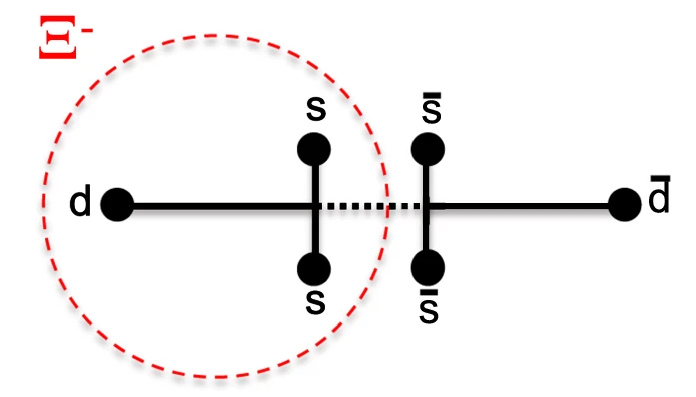
\includegraphics[width=0.55\textwidth, valign=t]{Figs/Chapter6/BaryonFormation_StringBreaking.png}
	\label{fig:StringBreaking}
} 
\subfigure[]{
	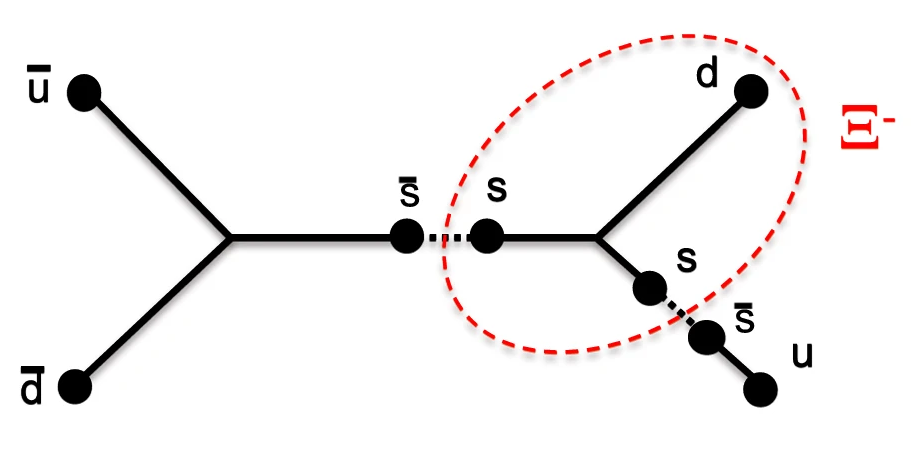
\includegraphics[width=0.6\textwidth, valign=t]{Figs/Chapter6/BaryonFormation_StringJunction.png}
	\label{fig:StringJunction}
} 
\caption{Baryon production mechanism within the \Pythia framework, in the case of a \rmXiM hyperon: (a) the colour string fragments into a diquark--anti-diquark pairs; (b) two strings form a junction, that breaks down into a $s\bar{s}$ pair. Figure taken from \cite{adolfssonQCDChallengesPp2020}.}
	\label{fig:BaryonProductionMechanisms}
\end{figure}

\Pythia has historically focused on electroweak and hard QCD processes, parton shower, hadronisation, particularly in small systems where no QGP formation is considered. The discovery of long-range particle correlations in high-multiplicity pp collisions in 2010 \cite{cmscollaborationObservationLongRangeNearSide2010}\cite{chatrchyanObservationLongrangeNearside2013}\cite{rolandLongrangeCorrelationsHigh2015}, followed by the observation of the strangeness enhancement in small systems in 2017 \cite{alicecollaborationEnhancedProductionMultistrange2017}, forced to re-consider the QGP-like effects in pp collisions. The aforementioned models could offer a qualitative description of some of those effects, while being completely off on some other observables like the anisotropic flow. New developments were needed. To that end, additional interactions between the strings have \say{recently} been implemented, namely the rope hadronisation (or also refered as colour rope) and string shoving \cite{bierlichComprehensiveGuidePhysics2022}.

The rope hadronisation follows somehow the same idea as the string junction, namely that strings may form in a cluster of partons. When multiple strings overlap, their colour field acts coherently, forming a stronger field. These cluster of strings can then be viewed as a string with an effective tension $\tilde{\kappa}$ greater than $\kappa$, that is a colour rope. This increased string tension leads to an increase\footnote{This increase actually depends on the colour configuration of the different strings. Quarks with the same colour charges can form a coherent state, increasing $\tilde{\kappa}$; whereas, with opposite/incoherent colour charges, they combine into an anti-colour, thus reducing $\tilde{\kappa}$.} of the strangeness production (or equivalently, it decreases its suppression factor), that can subsequently be used to model the strangeness enhancement.

Another effect of the overlapping of strings is the string shoving. Strings occupying the same volume can interact together. It turns out that they dominantly repel each other, resulting in a shoving pressure. Each hadron later receives its share of the push, which leads ultimately to a flow of hadrons, mimicing the anisotropic flow effects.

\subsubsection{\Epos}

Originally designed to reproduce heavy-ion interactions, \Epos employs a core-corona model, an unique approach when all the other high-energy physics MC generators (\Pythia, \Herwig, etc) are corona-like models. 

The basic idea behind this framework starts with the observation that a hadron-hadron collision corresponds in fact to many elementary collisions happening simultaneously, that can be modelled via the formation of parton ladders -- similar to the MPI concept, describing the multiple parton scatterings -- or (cut-)Pomerons\footnote{A Pomeron -- named after Isaak Pomeranchuk -- is a concept incorporated by Vladimir Gribov into the Regge theory, developed by Tullio Regge in 1959 \cite{reggeIntroductionComplexOrbital1959}. This theory attempts to describe the total cross section of hadronic collisions at high energies, at a time when the quark model does not exist yet. In this theory, a particle and all its excitations -- for instance, the \rhoMes meson spin-1, spin-3, spin-5, etc -- lie on the same trajectory, the Regge trajectory. Each resonance contributes to the scattering amplitudes; their combined contribution is viewed as an exchange of an object named Reggeon \cite{levinEverythingReggeonsPart1998}. Although the Regge theory provides a good description of the total cross section at low energies, it predicts a decreasing trend at high energies while it is in fact flat. The solution to this problem is brought by Gribov, who introduces a new Reggeon: the Pomeron. In modern particle physics, the Pomeron corresponds to various processes at high energy, such as a parton ladder. \Epos' main theoretical tool is the S-matrix theory, inspired by the Gribov-Regge picture \cite{wernerCorecoronaProcedureMicrocanonical2023}. One can distinguish two sorts of Pomeron: the cut and the uncut version. Basically, the latter corresponds to an elastic contribution to the scattering amplitude, whereas the former represents an inelastic contribution \cite{wernerMonteCarloEvent2022}.}. It turns out the parton ladder can be viewed as a colour flux tube, a string like in Lund string model that breaks via the production of a $q\bar{q}$ pair into string segments often referred as \say{pre-hadrons}. These serves as initial conditions for the hadronisation.

\begin{figure}[t]
\centering
	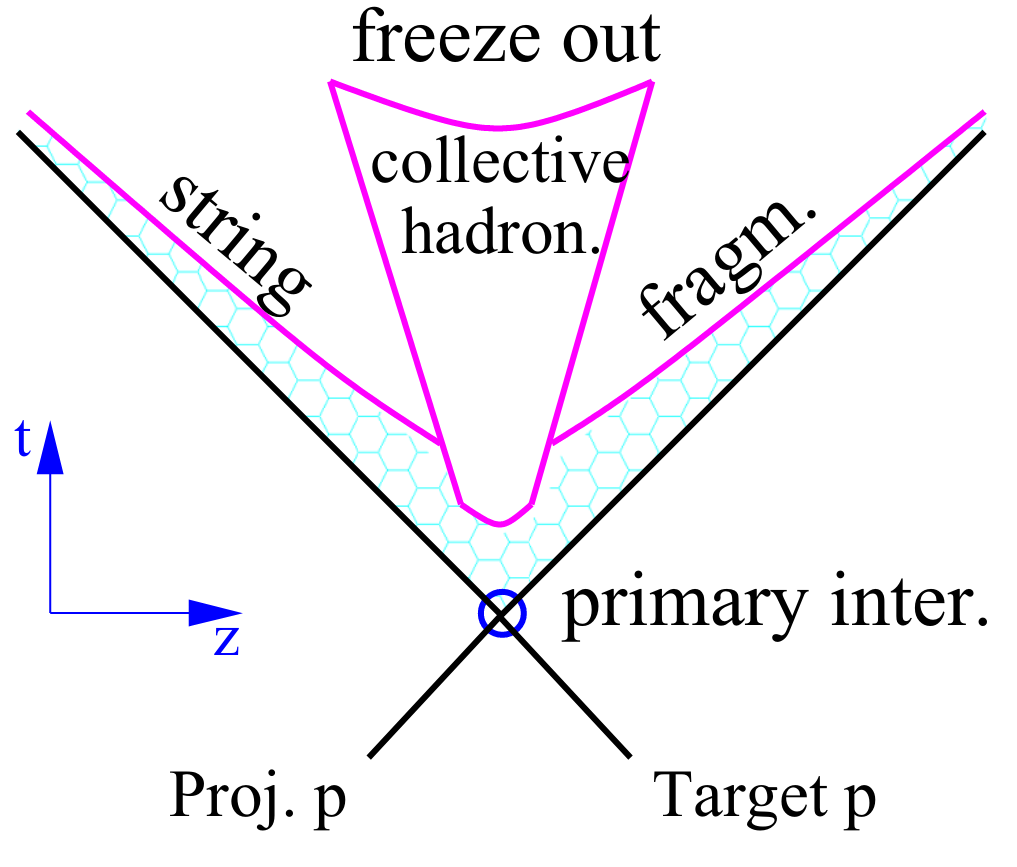
\includegraphics[width=0.55\textwidth, valign=t]{Figs/Chapter6/medium.png}
\caption{Schematic representation of the space-time evolution of the particle production in a hadron-hadron collision. The central cone represents the core part where the hadrons undergo a collective hadronisation at the freeze-out surface. The hyperbola line encompasses the corona surrounding the core; the string segments in this region  hadronise via string fragmentation. Figure taken from \cite{pierogEPOSLHCTest2015}.}
	\label{fig:CoreCorona}
\end{figure}

Based on these pre-hadrons, the core-corona procedure illustrated in \fig\ref{fig:CoreCorona} comes into play. In the regions with a high density (above a certain threshold, easily reached in heavy-ion collisions) of string segments, these may overlap and fuse into a fluid. This corresponds to the \say{core} of the system as opposed to the \say{corona}, usually located in the peripheral regions of the system (by definition), where the string density is lower. The pre-hadrons in the core lose their energy and evolve according to hydrodynamics, until the energy density falls below a critical value. At this stage, the fluid undergoes a collective hadronisation via a micro-canonical procedure\footnote{The string segments constituting the core are gathered in different clusters for each pseudo-rapidity bin. The hadronisation is performed in each cluster separately using the micro-canonical ensemble formalism \cite{pierogEPOSLHCTest2015}.} at the freeze-out surface (\fig\ref{fig:CoreCorona}), in order to ensure energy, momentum and flavour conservation. The formed hadrons receive a Lorentz boost according to the radial and longitudinal expansions of the fluid core. For what concerns the string segments in the corona part, they hadronise through string fragmentations as in \Pythia.\\

This presentation of \Epos corresponds to the current implementation of the model, \EposFour. This procedure is applied for simulating both pp and heavy-ion collisions. Thereby, this model assumes the formation of, at least, a QGP droplet in small systems (\fig\ref{fig:CoreCoronaPbPbpp}). There exists also different configurations that considers only \say{core} or \say{corona}.

\begin{figure}[t]
\centering
\subfigure[]{
	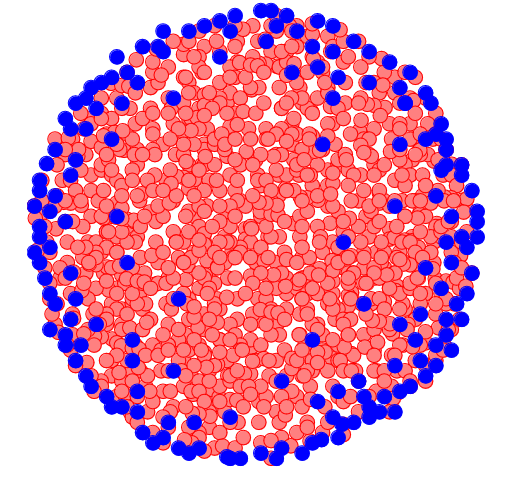
\includegraphics[width=0.35\textwidth, valign=t]{Figs/Chapter6/CoreCoronaPbPb.png}
}
\subfigure[]{
	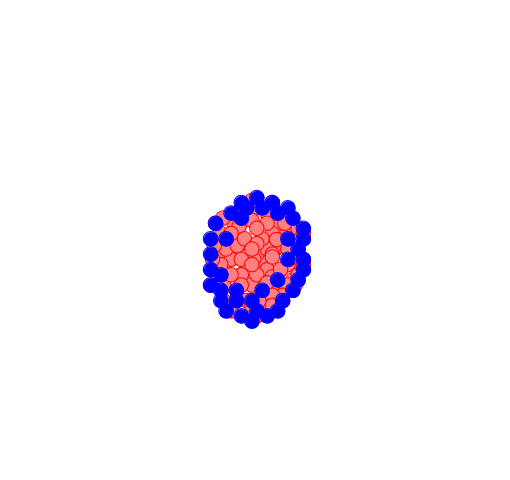
\includegraphics[width=0.35\textwidth, valign=t]{Figs/Chapter6/CoreCoronapp.png}
}
\caption{Schematic representation of the pre-hadrons distributions in a large system such as a Pb-Pb collision (a) and in a small system like a pp collision (b). The red dots represents the pre-hadrons in the core, while the blue ones belong to the corona. Figures taken from \cite{wernerCorecoronaProcedureMicrocanonical2023}.}
	\label{fig:CoreCoronaPbPbpp}
\end{figure}

\subsubsection{Comparison to the model predictions}

%\subsubsection{\Herwig}


